% Nội dung phần 2: Khám phá và tổng hợp dữ liệu (EDA).

\section{Khám phá và tổng hợp dữ liệu}

\subsection{Làm sạch dữ liệu}

Trước khi phân tích, nhóm chạy một bộ kiểm tra chất lượng trên toàn bộ 165.474
dòng. Kết quả được tổng hợp ở Bảng~\ref{tab:quality}: không có giá trị khuyết
thiếu, không có dòng trùng lặp hoàn toàn, không có session nào bị đứt quãng thứ
tự \texttt{order}, mọi session đều có đúng một click mang nhãn \texttt{Exit}, và
không có session nào bị chia cắt giữa hai tập dữ liệu.

\begin{table}[H]
\centering
\caption{Kết quả kiểm tra chất lượng dữ liệu}
\label{tab:quality}
\begin{tabular}{lr}
\toprule
\textbf{Kiểm tra} & \textbf{Số trường hợp vi phạm} \\
\midrule
Giá trị khuyết thiếu                 & 0 \\
Dòng trùng hoàn toàn                 & 0 \\
Session có \texttt{order} không liên tục & 0 \\
Session không có đúng một \texttt{Exit}  & 0 \\
Session xuất hiện ở cả train và test     & 0 \\
\bottomrule
\end{tabular}
\end{table}

Về chuyển đổi kiểu dữ liệu, các cột mã số nguyên có bản chất phân loại được
chuyển thành factor kèm nhãn đọc được: \texttt{country} (47 mức),
\texttt{category} (4 mức), \texttt{colour} (14 mức), \texttt{location} (6 mức),
\texttt{photography} (2 mức) và \texttt{page} (5 mức). Ba cột
\texttt{year}, \texttt{month}, \texttt{day} được ghép thành một biến ngày, từ đó
tạo biến thời gian liên tục \texttt{time\_30} tính theo đơn vị 30 ngày kể từ ngày
đầu tiên của dữ liệu.

Về dữ liệu ngoại lai, nhóm \textbf{không} xóa và cũng không winsorize các session
dài, dù chúng nằm xa ngoài râu boxplot (\texttt{order} lớn nhất là 195). Lý do là
các session này có trình tự \texttt{order} hoàn toàn hợp lệ và phản ánh hành vi
duyệt dài có thật, không phải lỗi ghi nhận. Thay vì loại dữ liệu hợp lệ, nhóm xử
lý phần đuôi phải bằng phép biến đổi $\log_2(\texttt{order})$ trong LPM/Logistic
và bằng hàm trơn trong GAM.

\subsection{Thống kê mô tả}

Cần phân biệt hai đơn vị phân tích khác nhau. Phân phối \texttt{order} được tính
trên toàn bộ click, còn phân phối độ dài session được tính ở cấp session. Vì các
session dài đóng góp nhiều click hơn vào tổng thể, không được dùng trung vị
\texttt{order} trên click để kết luận về một session điển hình.

\begin{table}[H]
\centering
\caption{Thống kê mô tả các biến định lượng}
\label{tab:continuous}
\small
\begin{tabular}{llrrrrrrrr}
\toprule
\textbf{Biến} & \textbf{Đơn vị} & \textbf{N} & \textbf{Mean} & \textbf{Median}
& \textbf{Q1} & \textbf{Q3} & \textbf{Min} & \textbf{Max} & \textbf{SD} \\
\midrule
Price          & Click   & 165.474 & 43,80 & 43 & 33 & 52 & 18 & 82 & 12,55 \\
Order          & Click   & 165.474 & 9,82  & 6  & 2  & 12 & 1  & 195 & 13,48 \\
Session length & Session & 24.026  & 6,89  & 4  & 2  & 8  & 1  & 195 & 9,00 \\
\bottomrule
\end{tabular}
\end{table}

Giá sản phẩm chỉ nhận 20 mức rời rạc từ 18 đến 82 USD, nên phân phối có nhiều
đỉnh; việc trung bình (43,80) gần trung vị (43) \emph{không} đủ để kết luận biến
này tuân theo phân phối chuẩn. Ngược lại, độ dài session lệch phải rất mạnh:
trung vị chỉ 4 click trong khi trung bình là 6,89; có 2,48\% session dài hơn 30
click và 0,071\% session dài hơn 100 click.

\begin{table}[H]
\centering
\caption{Bảng tần số các biến phân loại chính}
\label{tab:categorical}
\small
\begin{tabular}{llrr}
\toprule
\textbf{Biến} & \textbf{Nhóm} & \textbf{Số click} & \textbf{Tỷ lệ} \\
\midrule
\multirow{4}{*}{Category}
 & Trousers & 49.742 & 30,06\% \\
 & Skirts   & 38.408 & 23,21\% \\
 & Blouses  & 38.577 & 23,31\% \\
 & Sale     & 38.747 & 23,42\% \\
\midrule
\multirow{6}{*}{Location}
 & Top left      & 34.532 & 20,87\% \\
 & Top middle    & 33.383 & 20,17\% \\
 & Top right     & 21.656 & 13,09\% \\
 & Bottom left   & 27.377 & 16,54\% \\
 & Bottom middle & 27.783 & 16,79\% \\
 & Bottom right  & 20.743 & 12,54\% \\
\midrule
\multirow{2}{*}{Photography}
 & En face & 122.439 & 73,99\% \\
 & Profile & 43.035  & 26,01\% \\
\midrule
\multirow{2}{*}{Price group}
 & A: Không cao hơn TB & 80.779 & 48,82\% \\
 & B: Cao hơn TB       & 84.695 & 51,18\% \\
\midrule
\multirow{5}{*}{Page}
 & Page 1 & 93.452 & 56,48\% \\
 & Page 2 & 41.037 & 24,80\% \\
 & Page 3 & 19.301 & 11,66\% \\
 & Page 4 & 8.861  & 5,35\% \\
 & Page 5 & 2.823  & 1,71\% \\
\bottomrule
\end{tabular}
\end{table}

Hai nhóm giá gần cân bằng về số lượng (48,82\% so với 51,18\%), thuận lợi cho
việc ước lượng chênh lệch với sai số chuẩn nhỏ. Tuy nhiên, cân bằng về \emph{cỡ
mẫu} không biến dữ liệu quan sát thành một thí nghiệm ngẫu nhiên -- điều này sẽ
được kiểm chứng bằng balance diagnostics ở Mục~\ref{subsec:ab}.

Phân phối \texttt{page} rất lệch: hơn một nửa số click nằm ở trang 1 và chỉ
1,71\% ở trang 5. Đây là lý do \texttt{page} được giữ ở dạng factor thay vì xem
như biến liên tục.

\subsection{Trực quan hóa dữ liệu}

\begin{figure}[H]
\centering
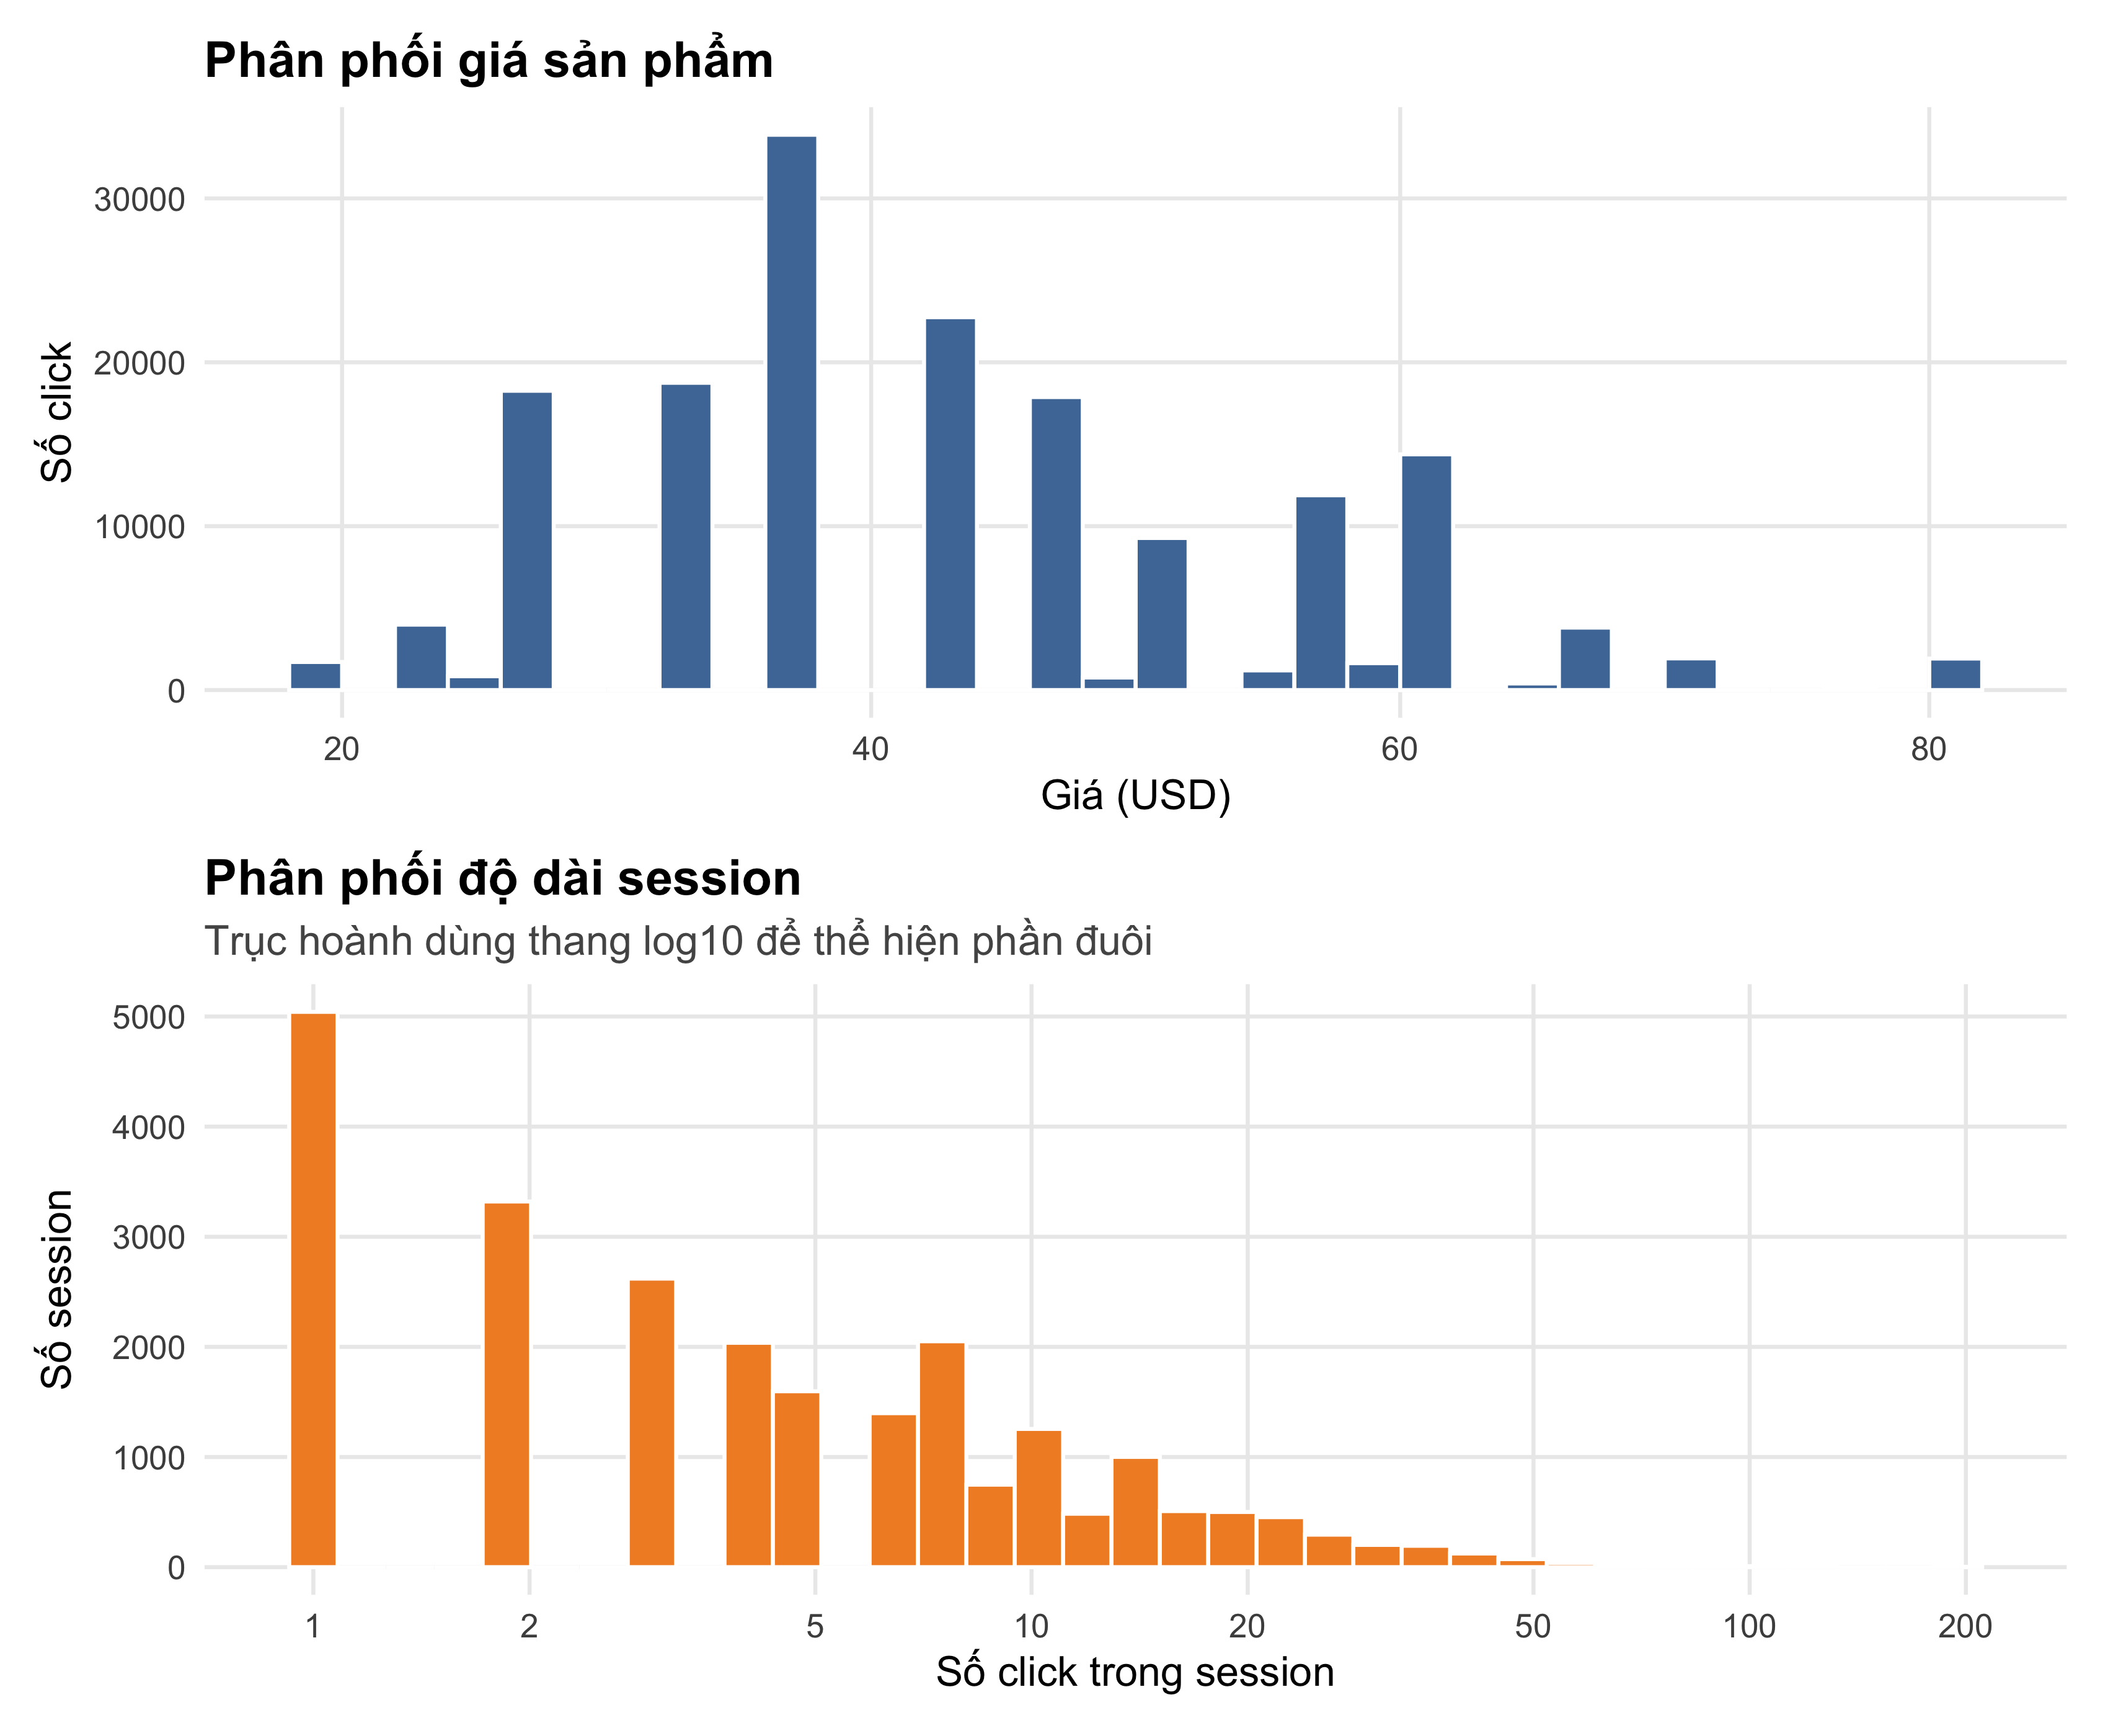
\includegraphics[width=\textwidth]{img/fig-eda-distributions.png}
\caption{Phân phối giá sản phẩm và phân phối độ dài session (trục hoành thang
log10)}
\label{fig:eda-distributions}
\end{figure}

Hình~\ref{fig:eda-distributions} cho thấy phân phối giá có dạng răng cưa, phản
ánh đúng bản chất rời rạc của các mức giá niêm yết. Phân phối độ dài session lệch
phải mạnh: phần lớn session rất ngắn, nhưng một tỷ lệ nhỏ kéo dài hàng chục đến
gần 200 click. Đây chính là căn cứ thực nghiệm cho quyết định dùng
$\log_2(\texttt{order})$ và hàm trơn thay vì cắt bỏ phần đuôi.

\begin{figure}[H]
\centering
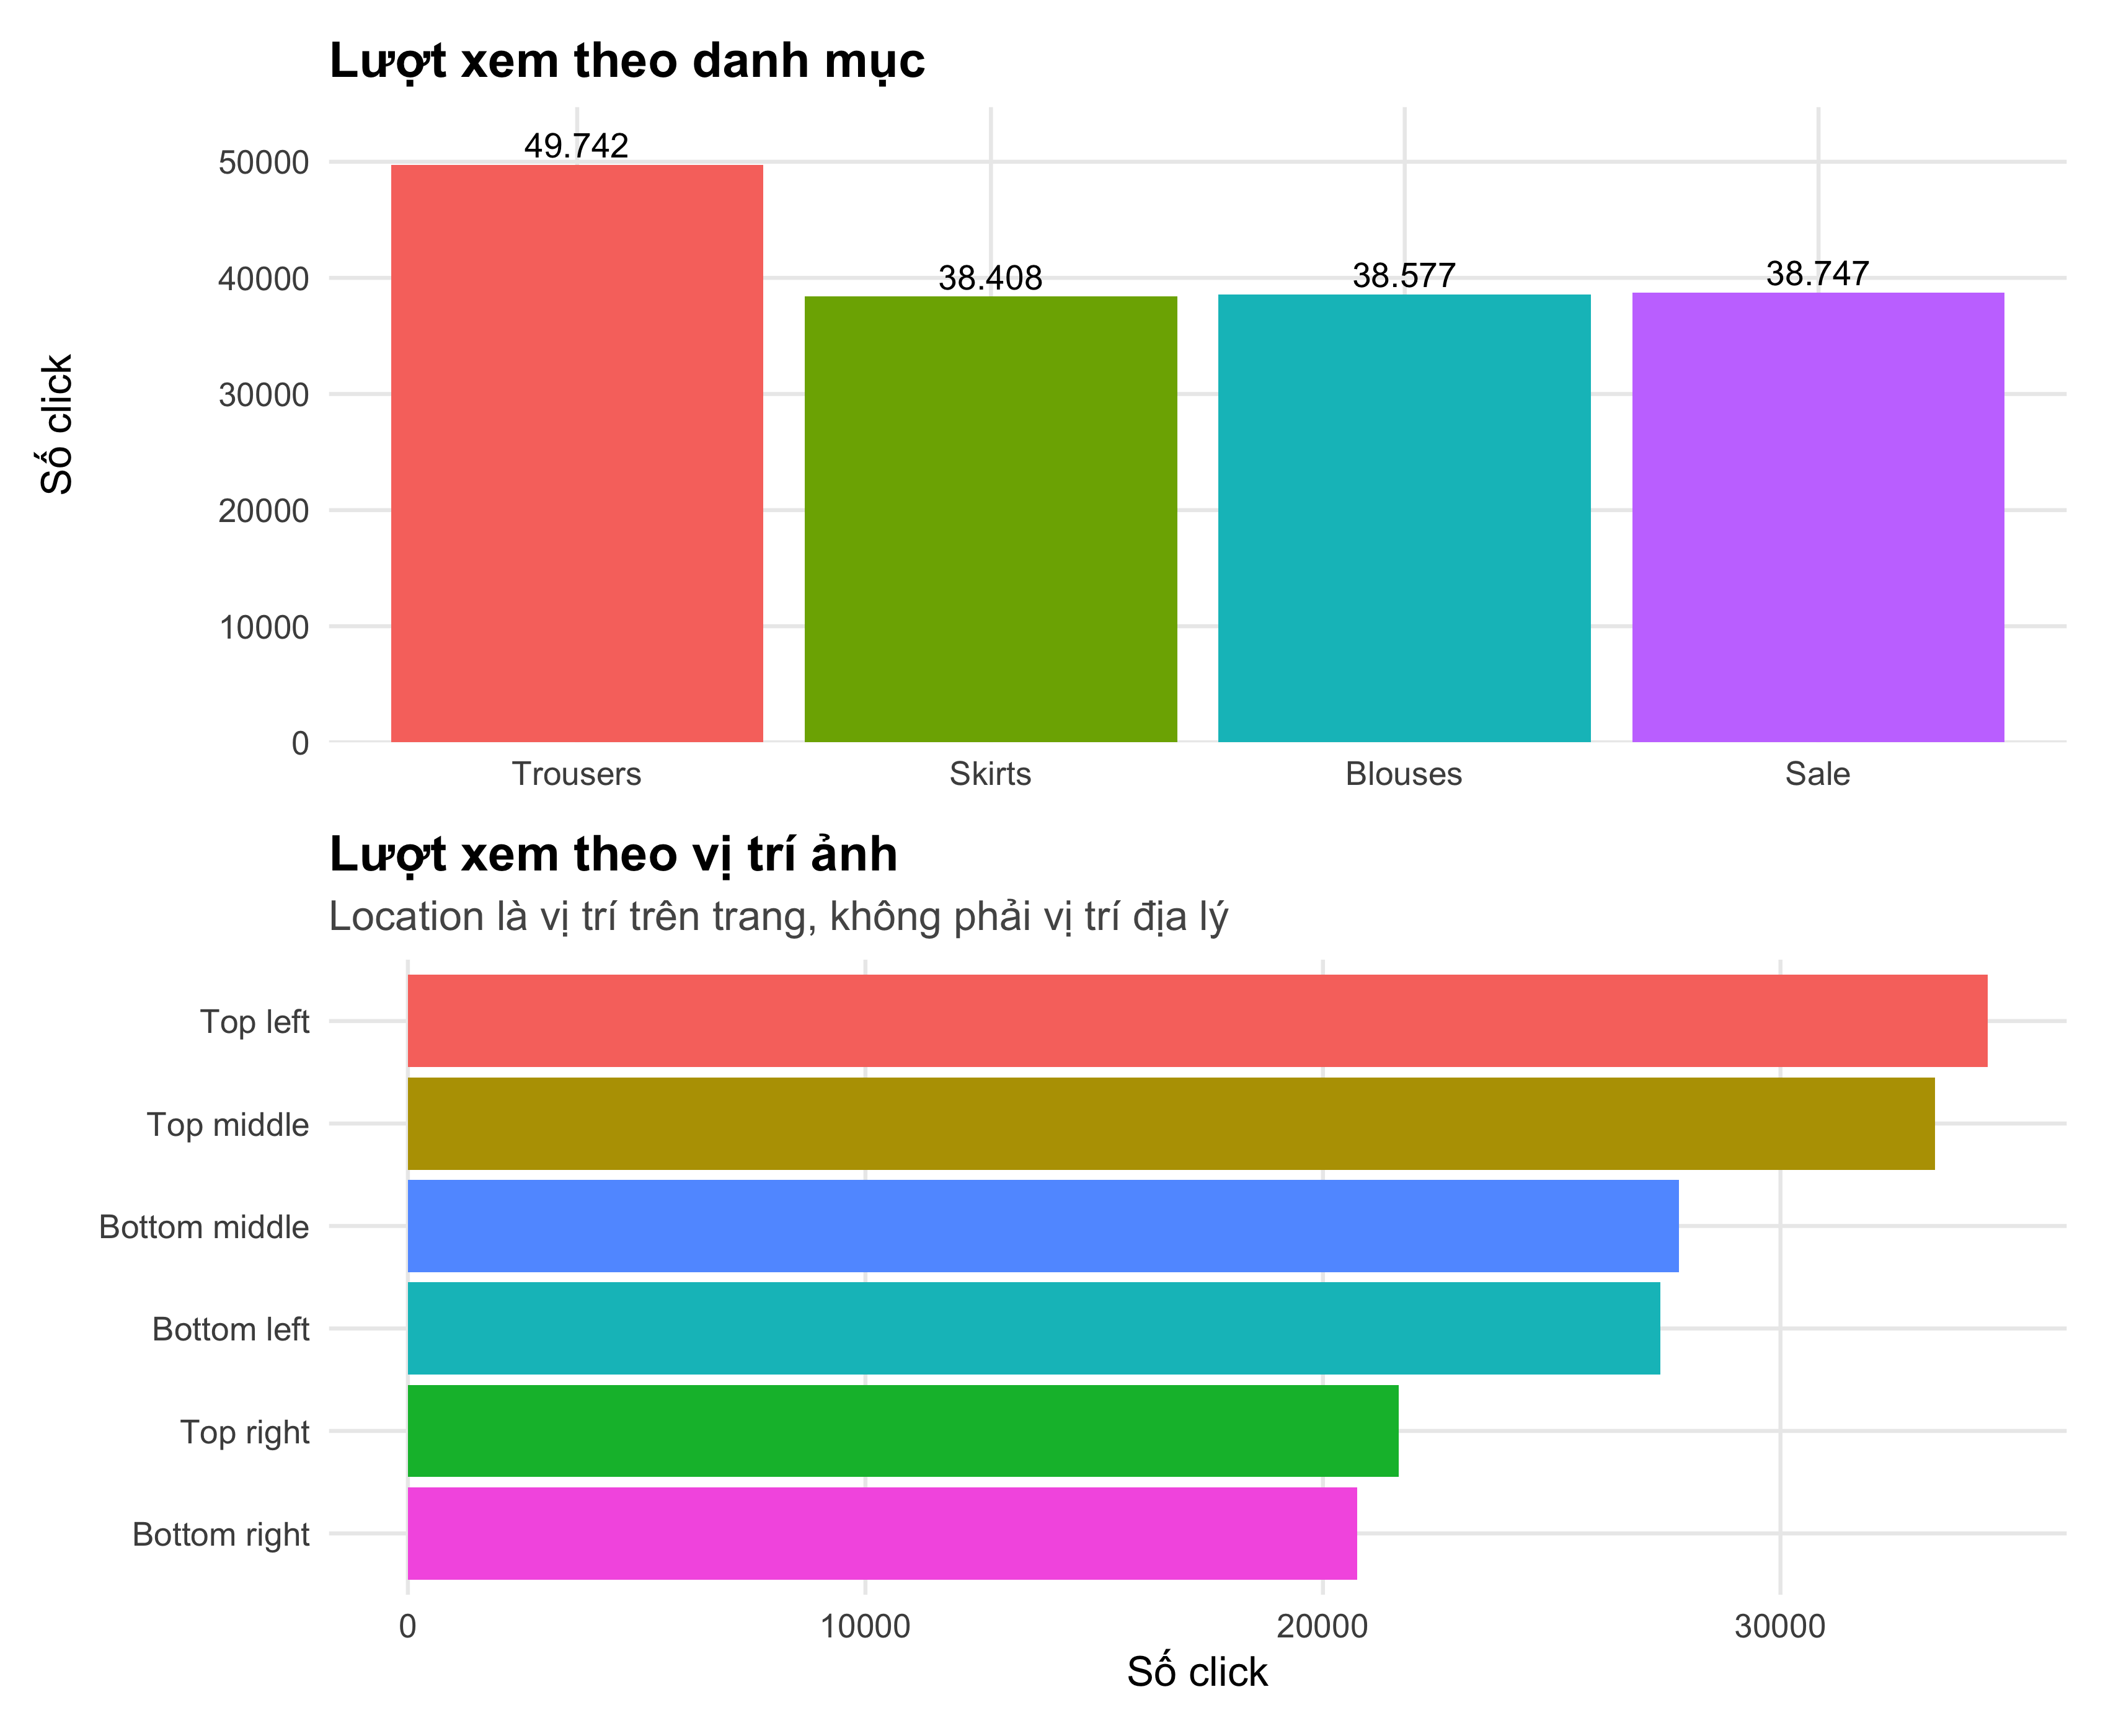
\includegraphics[width=\textwidth]{img/fig-eda-categories.png}
\caption{Số lượt click theo danh mục sản phẩm và theo vị trí ảnh trên trang}
\label{fig:eda-categories}
\end{figure}

Danh mục Trousers có số click cao hơn rõ rệt so với ba danh mục còn lại
(30,06\% so với khoảng 23\% mỗi nhóm). Đây chỉ là mô tả lưu lượng xem, chưa đủ để
kết luận danh mục này hấp dẫn hơn hay tạo chuyển đổi tốt hơn. Tương tự, các vị
trí ảnh có tần số khác nhau, nhưng vì mỗi mã sản phẩm chỉ xuất hiện tại một vị
trí cố định, khác biệt theo \texttt{location} có thể bị confounding hoàn toàn bởi
đặc điểm sản phẩm.

\begin{figure}[H]
\centering
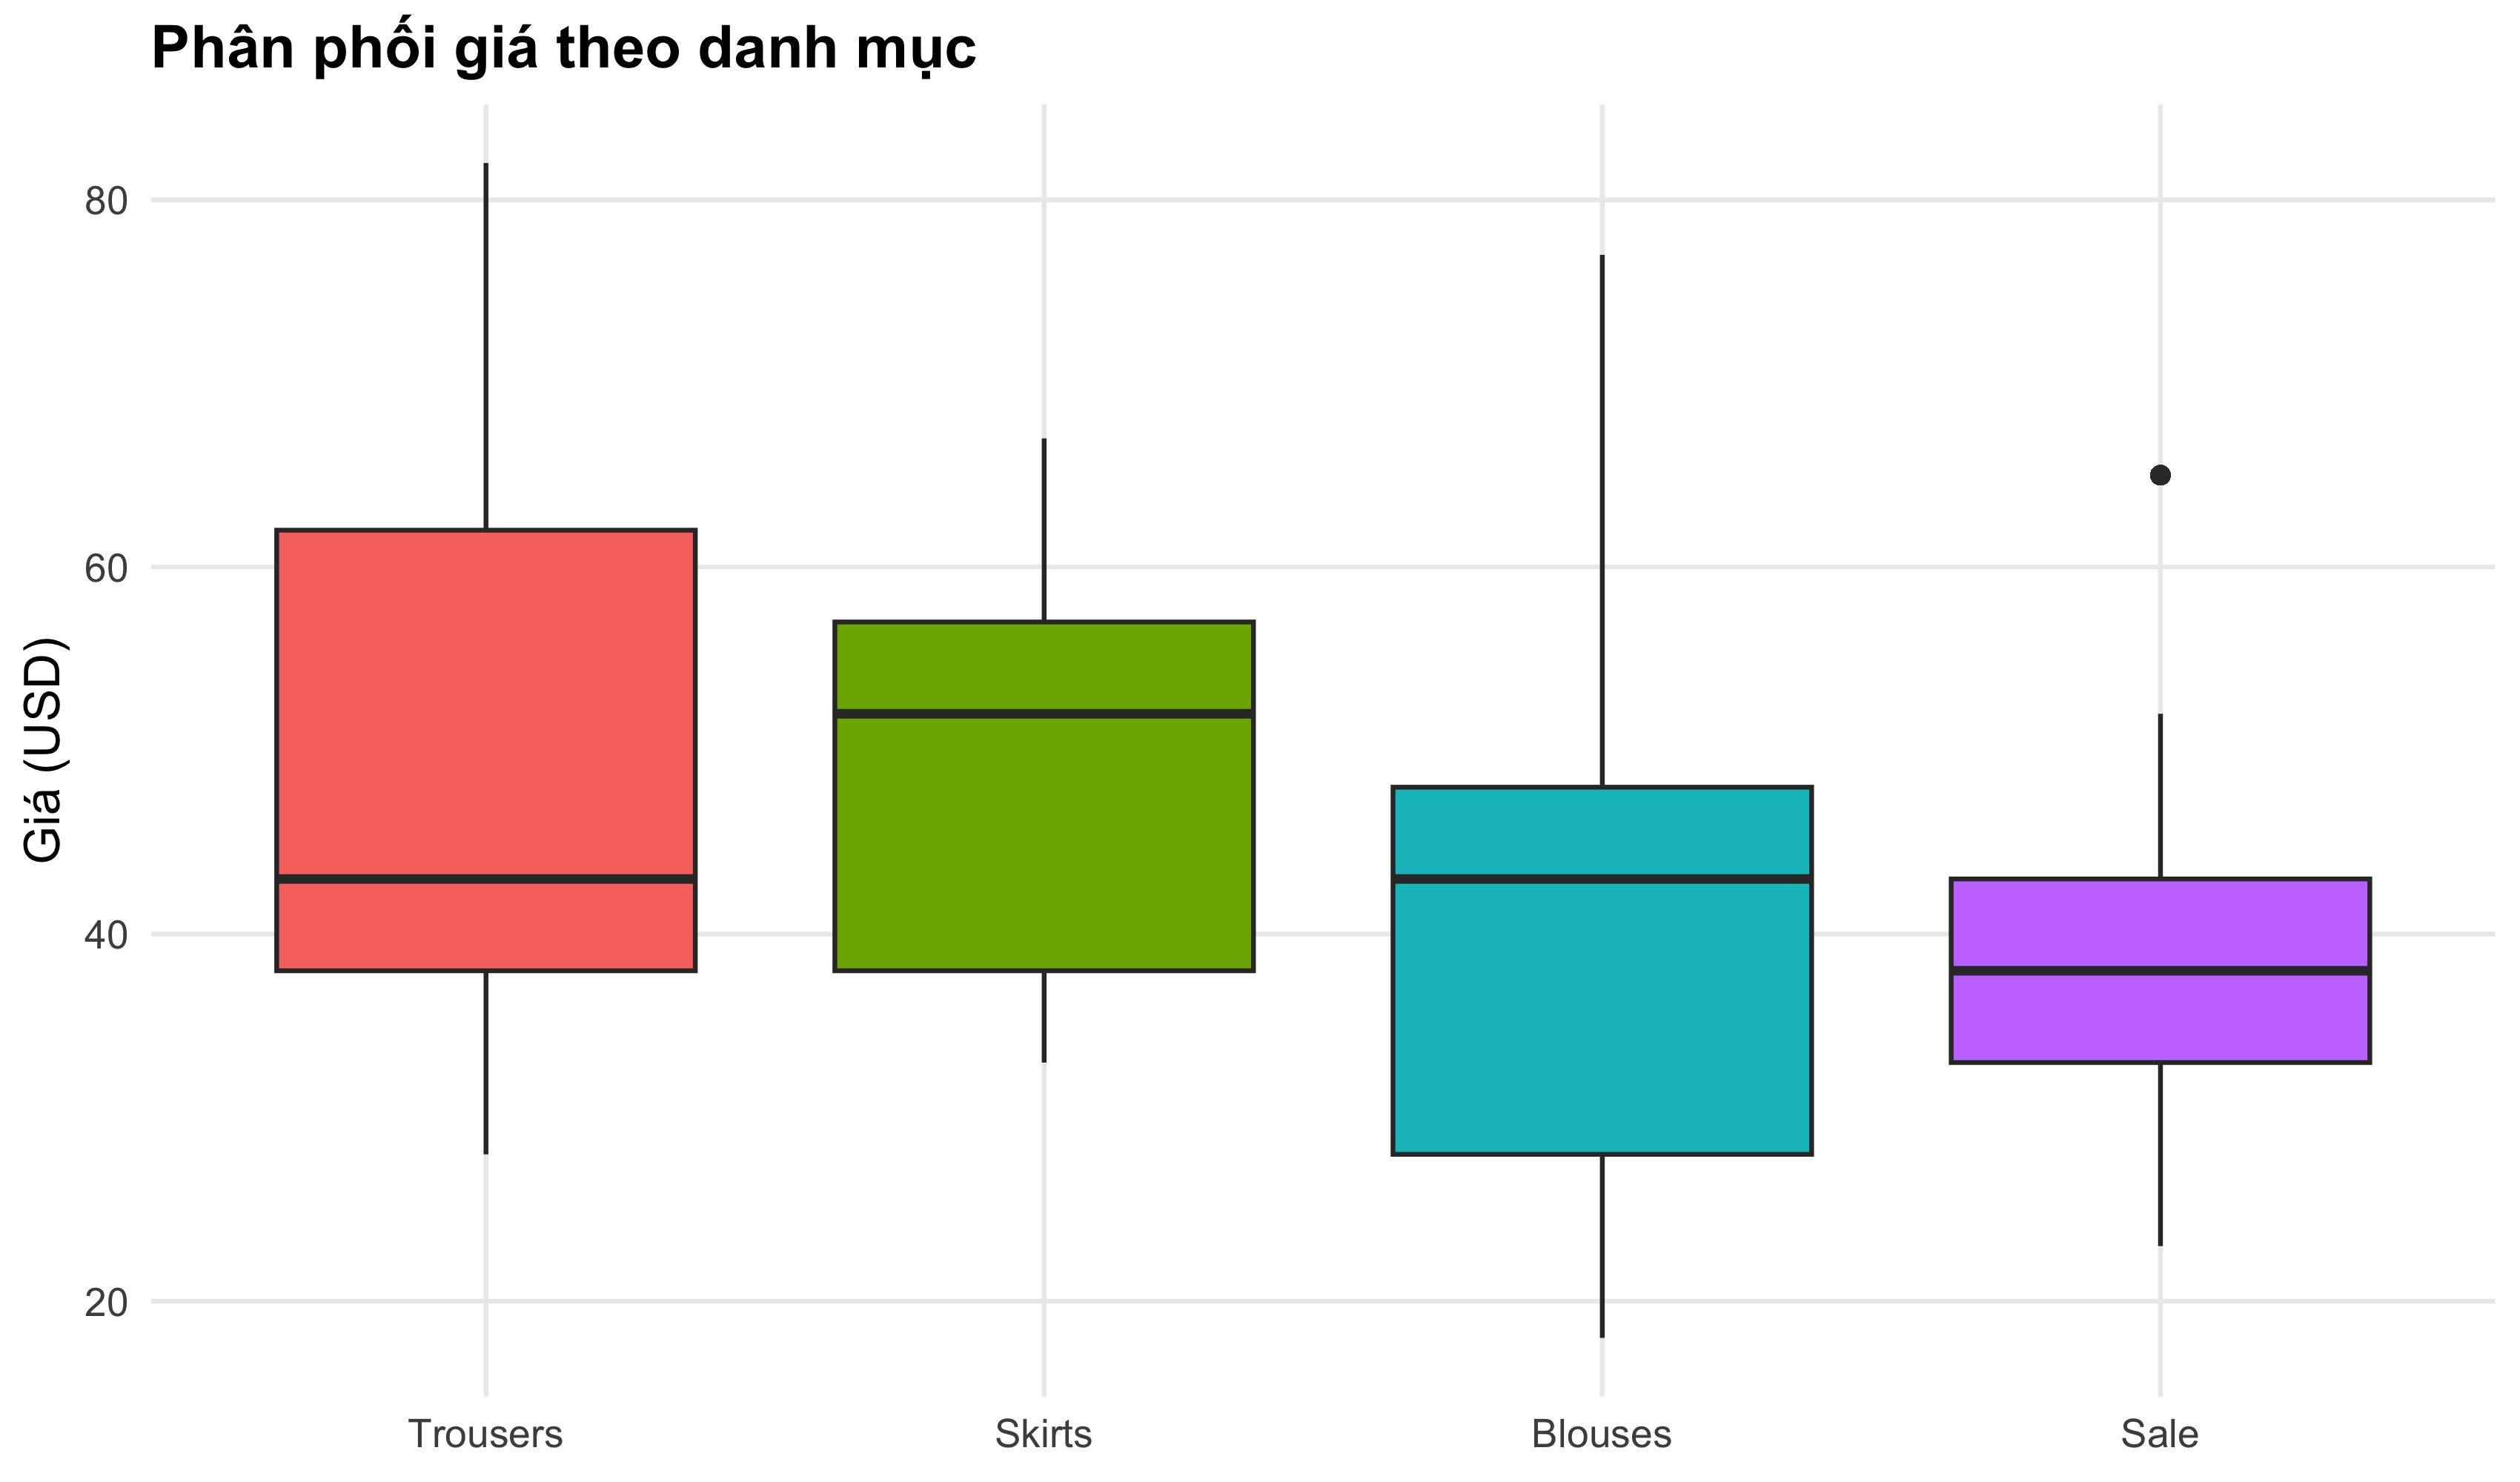
\includegraphics[width=0.85\textwidth]{img/fig-eda-price-category.png}
\caption{Phân phối giá theo danh mục sản phẩm}
\label{fig:eda-price-category}
\end{figure}

Hình~\ref{fig:eda-price-category} cho thấy mặt bằng giá khác biệt rõ giữa bốn
danh mục. Vì biến \texttt{price\_above\_avg} được xác định theo trung bình của
\emph{chính danh mục đó}, mọi phân tích so sánh hai nhóm giá bắt buộc phải kiểm
soát \texttt{category}, và không được xem nhóm giá là một treatment được ngẫu
nhiên hóa.

\begin{figure}[H]
\centering
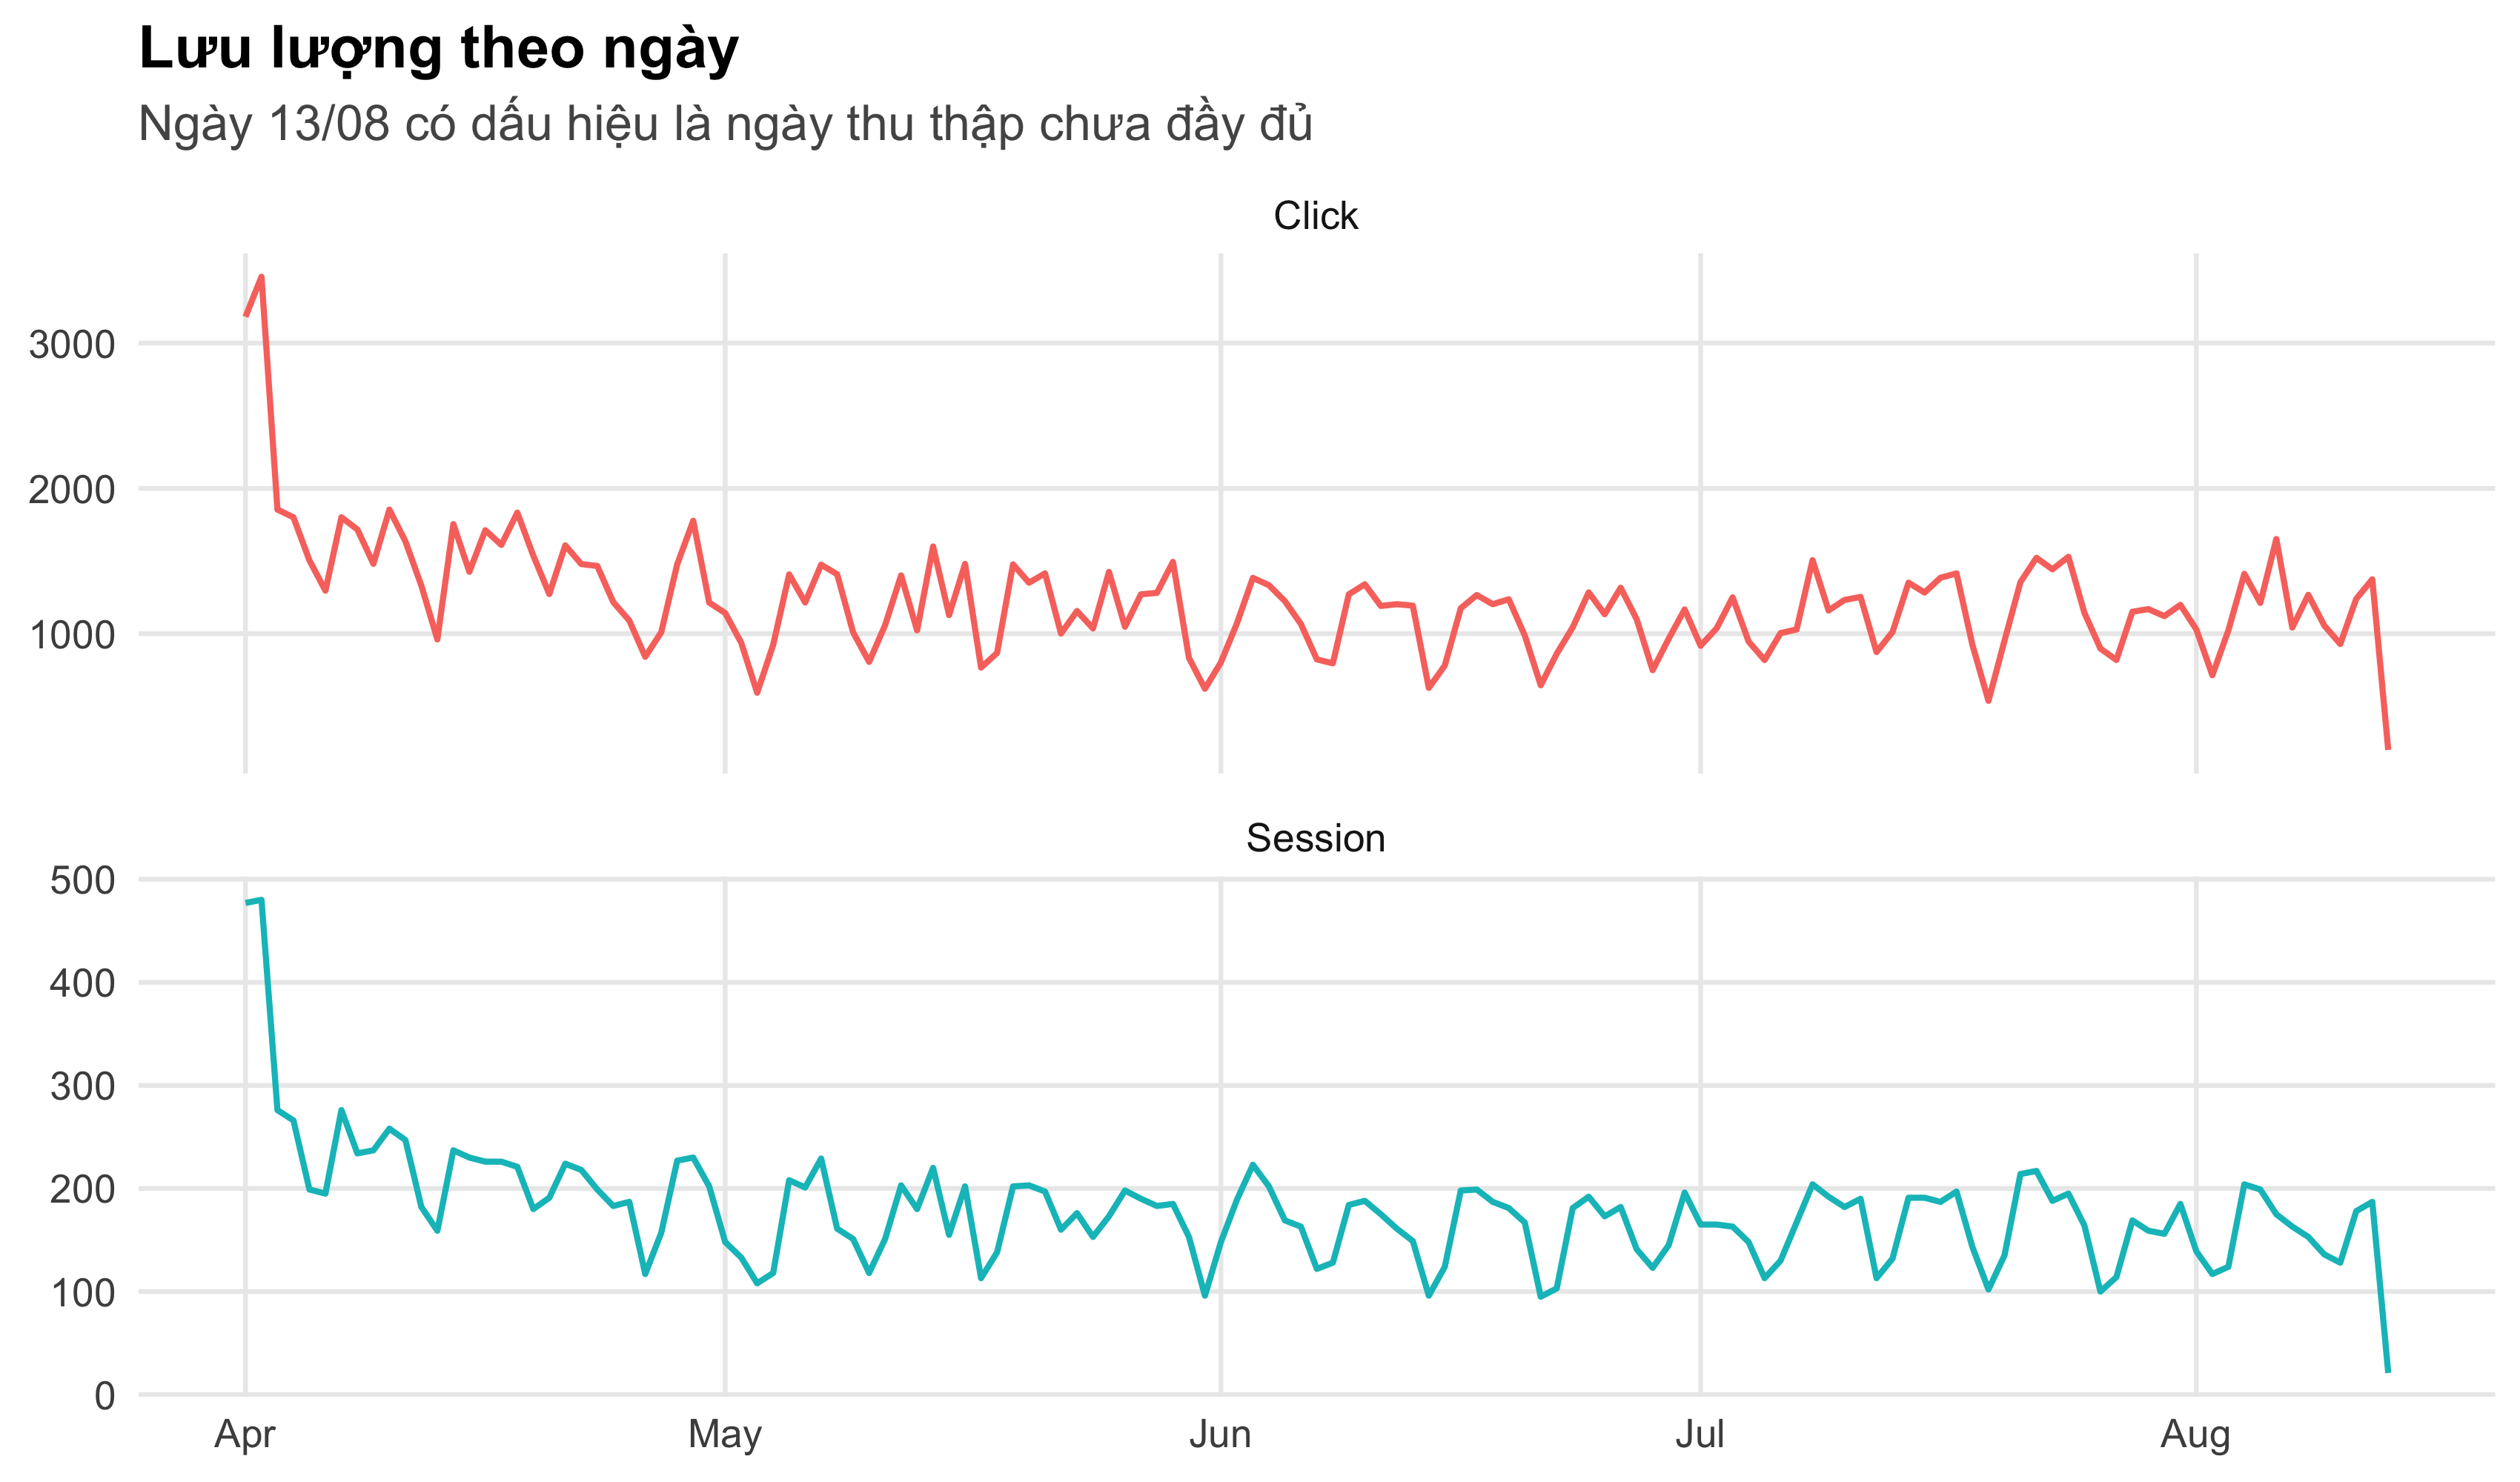
\includegraphics[width=\textwidth]{img/fig-eda-time.png}
\caption{Lưu lượng click và số session theo ngày}
\label{fig:eda-time}
\end{figure}

Chuỗi thời gian ở Hình~\ref{fig:eda-time} cho thấy lưu lượng biến động rõ theo
ngày và theo tuần, củng cố quyết định chia dữ liệu theo thời gian thay vì ngẫu
nhiên. Điểm sụt mạnh ở cuối chuỗi ứng với ngày 13/08 chỉ có 200 click, dấu hiệu
của một ngày thu thập dở dang chứ không phải bằng chứng về suy giảm lưu lượng
thực sự.

Nhóm cố ý \emph{không} trình bày ma trận tương quan Pearson cho toàn bộ các cột,
vì phần lớn biến trong bộ dữ liệu là mã factor (country, colour, location,
page\ldots); hệ số tương quan tính trên các mã số này không có ý nghĩa thống kê.
Quan hệ giữa các biến phân loại và \texttt{Exit} được đánh giá trực tiếp bằng các
mô hình ở Phần~\ref{sec:results}.
